\section{Analysis of a visualization} 

\begin{figure}
 \centering % avoid the use of \begin{center}...\end{center} and use \centering instead (more compact)
 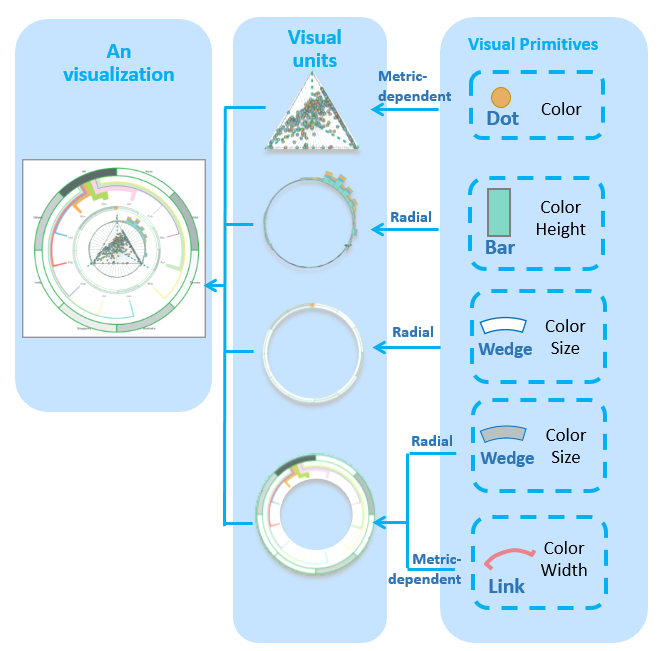
\includegraphics[width=\columnwidth]{hierarchic}
 \caption{An example of the hierarchical structure of a visualization, Opinion Seer\cite{wu_opinionseer:_2010}}
 \label{fig:hierarchic}
\end{figure}




\subsection{Compositions of a visualization}
Previous works have proven that learning by constructin is effective for grasping new knowledge.\cite{huron_constructive_2014, chapman_constructive_1988}  We incorporate the lessons from previous work\cite{munzner_visualization_2014, huron_constructive_2014, chi_taxonomy_2000}  with our observation, define the compositions of a visualization and the relationships between these compositions. 

\subsubsection{Hierarchical structure}
We propose a model that decomposes a visualization into three levels of structure: visual primitives, visual units, and then an advanced visualization design. 

\textbf{A visual primitive} is one graphic element whose visual channels are mapped to data attributes. We employ the defination in previous work\cite{huron_constructive_2014, satyanarayan_vega-lite:_2017}, use the term "grammar" to describe how the visual appearance of a visual primitive is influenced by data. For instance, a point whose size and color are encoded is a visual primitive. How the two visual channels, size and color, are related to data attributes is its visual grammar. 

\textbf{A visual unit} is the assembly of visual primitives based on a certain construction rule, as tab.1 show. We are not prentending that this table includes all existing visual uints, since new design is proposed constantly. A visual unit is the smallest functional unit of a visualization. A bubble chart, which groups the points mentioned above in an orthogonal coordinate, is a visual unit. A Venn diagram, which is also a visual unit, assembles dots in a metric-dependent way.  Note that people might employ two visual primitives in a novel visualization design. For example, \textit{Visual Sedimentation}\cite{huron_visual_2013} employs two visual primitives, bar and dot, to construct a novel design. 

\textbf{An visualization} can be treated as the combination of visual units. An naive visualization can be as simple as one visual unit while an advanced one is usually the combination of several units. But it doesn't simply put all visual units together but construct them with certain connections with each other, which is detailedly discussed in section 3.1.2.



\begin{figure}
\begin{minipage}{\columnwidth}
 \centering % avoid the use of \begin{center}...\end{center} and use \centering instead (more compact)
 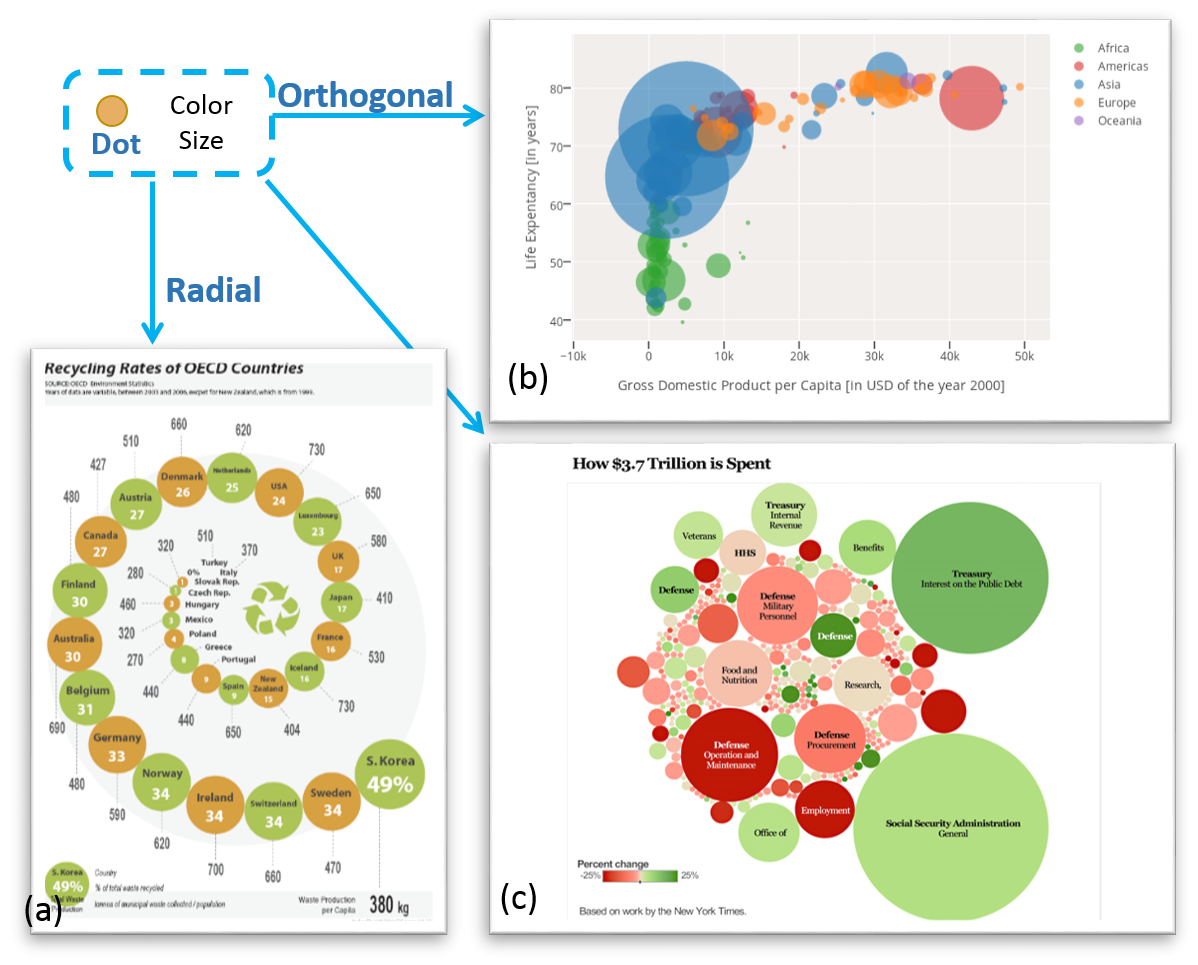
\includegraphics[width=\columnwidth]{assemble}
\caption[assemble]
{ A dot, whose color and size are encoded, can assemble 
(a) a dot spiral chart
\protect\footnotemark{}
    , (b)a dot packing chart
  \footnotemark{}
  , and (c)a bubble chart
  \footnotemark{}
   by following different construction rules.
}
\end{minipage}
\label{fig:hierarchic}
\end{figure}
\footnotetext{https://www.pinterest.com/pin/16536723602037537/}
\footnotetext{https://plot.ly/~etpinard/84.embed}
\footnotetext{https://bl.ocks.org/mbostock/4063269}

\begin{table}[tb]
  \caption{A taxonomy of visual units.}
  \label{tab:unit}
  \small
  \centering
  \begin{tabular}{p{0.8cm}|p{1.8cm}|p{2.0cm}|p{2.4cm}}
  \toprule
 \textbf{} &\textbf{Radial} & \textbf{Orthogonal} & \textbf{Metric-dependent}   \\ 
  \midrule
  \textbf{Line} &Spiral Line & Line Chart & \\ 
  \midrule
  \textbf{Area} & &Area Graph  & Treemap, Flow Map \\ 
  \midrule
  \textbf{Bar} &Radial Bar Chart, Sunburst Diagram & Bar Chart & \\
  \midrule
  \textbf{Dot} & &Scatter Plot, Bubble Chart &Bubble Map \\
  \midrule
  \textbf{Wedge} & Pie Chart, Donut Chart &Arc Diagram & \\
  \midrule
  \textbf{Link} &Chord Diagram &Parallel Coordinates &Node-link Diagram \\
  \midrule
  \textbf{Text} & &Parallel Tag Cloud [] &Word Cloud \\
  \midrule
  \textbf{Image} & &Heatmap Matrix &Heatmap \\

  \bottomrule

  \end{tabular}
  \vspace{1mm}
\end{table}

\subsubsection{Relationships between visual units}
An advanced visualization is often the combination of several visual units. Through observing the approaches people apply to design new visualizations, we define four types of relationship between visual units in our model: irrelevance, relevance, enhancement, and dependency. 

\textbf{Irrelevance} refers to that two visual units have no correlations in their visual encodings. It is a bi-directional relation. As in \textbf{figure1a}, 2 donut charts are applied to illustrate the distribution of age and gender groups respectively in a population. They are put together just for space-efficiency and there is no correlation between these two charts. 

\textbf{Relevance} refers to that two visual units share some encoding scheme, and it is a bi-directional relation. For example, in \textbf{figure 1b}, bar chart and line chart show the same encoding of horizontal position. According to our survey, color and position are the most commonly shared visual encodings, which might be the result that color and position usually encoded with simple while crucial information. 

\textbf{Enhancement} is an one-way relationship. If one visual unit A is the enhancement of another visual unit B, it means that A is imported to B, replaces some graphic elements of B and thus enables the representation of some data attributes that B alone fails to convey. Suppose there are 5 types of area in a park. A bar chart illustrates their average price per unit area, a chord diagram illustrates how passengers travel through each area. Then, as in \textbf{figure 1c}, the bar chart take the place of node segments in chord diagram, resulting in a novel and informative visualization. Some actual examples are the heat map mapped upon the steams in a theme river\cite{wu_opinionseer:_2010}  and usage of glyphs to enhance the meaning of nodes in a multidimensional scaling plot.\cite{chen_peakvizor:_2016}

\textbf{Dependence} is an one-way relationship. If one visual unit A is dependent on B, it means that A is added to B to reveal some information that results from the visualization B adopts to a dataset. The biggest difference between "\textbf{enhancement}" and "\textbf{dependence}" is that \textbf{enhancement} illustrate the data attributes in the data set, while \textbf{dependency} reveals the new knowledge we obtain from adopting a visualization a dataset. For example, in \textbf{figure xxx}, a multiple dimensional scaling (MSD) map shows the similarity between each restaurants in a city. A heat map is then added to the MSD map to show the most common type of restaurants, which information can hardly be obtained from the dataset but quite evident from the previous visualization. 
\subsubsection{Correlations between visual primitives}
The inner relationship between visual primitives is relatively simple.
A visual unit, which is the smallest function unit in a visualization, rarely have more than 2 visual primitives. And the relationship between the 2 visual primitives, if there are two, are quite obvious. The encoding of one primitive always has a high dependency on the encoding of another primitive. For example, in a chord diagram, the encoding of the arcs should be explained before the line connecting them. 


\begin{figure}[tb]
 \centering % avoid the use of \begin{center}...\end{center} and use \centering instead (more compact)
 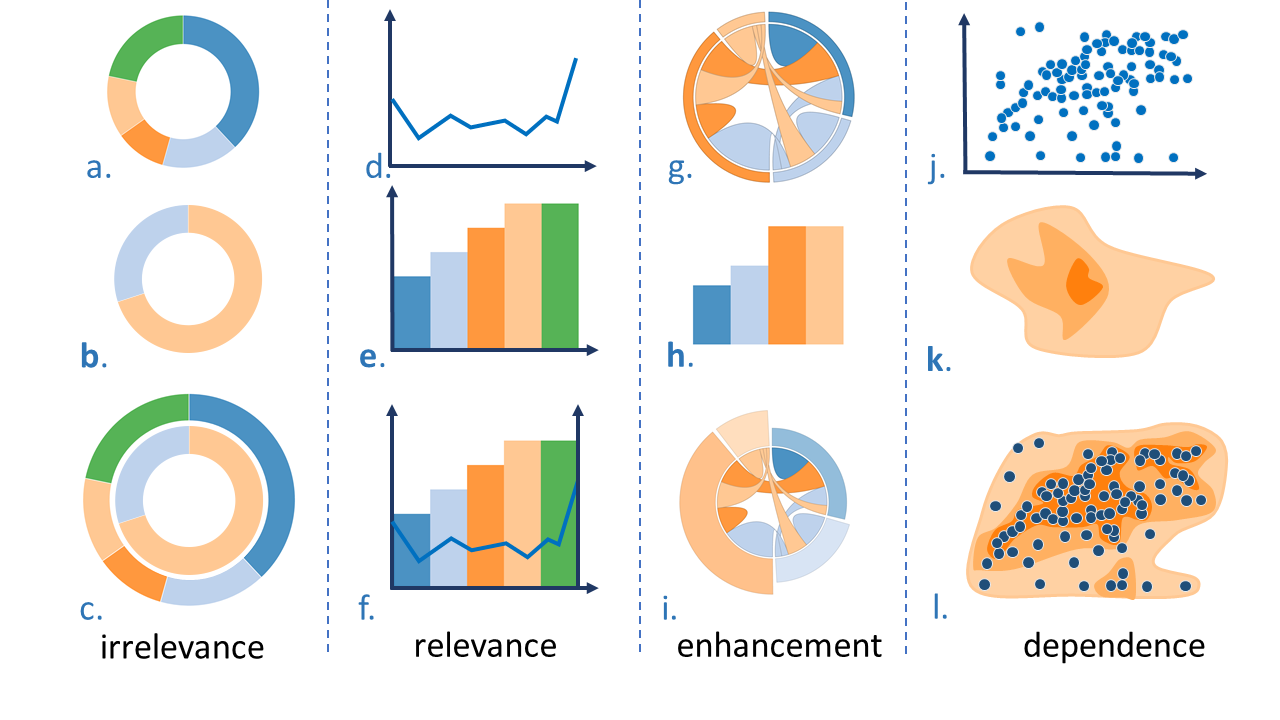
\includegraphics[width=\columnwidth]{unit_relationship}
 \caption{Illustration of the 4 types of relationship between visual units}
 \label{fig:relationship}
\end{figure}

\subsubsection{Correlations between visual channels}
The relationship between channels might be the most complicated relationship in our model. Since different channels are encoded with different information, they are usually separated and have no logic dependency upon others. However, an arbitrary explaining order of visual channels may lead to an unefficient information delivery, especially when a mark has multiple channels, which is common in an advanced visualization. 

Therefore, we define two metrics to order the explaining of visual channels: \textbf{the complexity of their encoded information} and \textbf{saliency of their visual appearance}.

First, a proper explanation should follow the order of decreasing visual saliency.\cite{cleveland_graphical_1984} Even though different channels have intrinsically different perceptual salience and channel with high salience will suppress the expression of other, such salience strength can be influenced in a task-dependent manner. \cite{nothdurft_salience_2000} By introducing the channel with high saliency first, we remove it from the task list in our mind, decrease its saliency and give other channels more chance to attract limited human attention. (maybe introduce some concepts such as salience map, pre-attentive stage, and focused attention stage) \par
 Second, we should follow the order of increasing complexity. “Easy to difficult” practice has been long used and confirmed to be effective for learning new tasks\cite{bliss_effects_1992}.\par
 Based on our survey, there are five common visual channels: color hue, size, position, shape, color saturation. Sorted in the increasing complexity order, it is color hue-color saturation-position-size-shape, while sorted in the decreasing visual saliency order, it is position-color hue-size-shape-color saturation \cite{munzner_visualization_2014,cleveland_graphical_1984}.  \par
In our system, we choose position-color hue-color saturation-size-shape as a trade-off between these two metrics. But we do allow and recommend the users to define their preferable sequence based on their situation. 

\subsection{Analysis of existing visual distraction}
We aims to introduce a new visualization design in a visual method, more specifically, in the form of a slide show. To better inform the crafting an attractive and effective explanation, analyzing the existing visual distraction is necessary. 
\textbf{add a fig}
From our observation, we identify two kinds of visual distractions: visual distraction from context and visual distraction from sibling channels (sibling channels refer to the channels belonging to the same mark). \par

\subsubsection{Visual distraction from the context}
This kind of distraction has been widely discussed in the field of object detection and human visual attention. \cite{nothdurft_salience_2000, standage_modelling_2005}Its intensity is mainly  determined by spatial distance and appearance similarity. \cite{wolfe_guided_1994}For example, when we try to focus on a green rectangel, a red triangel near by it can lead to visual distraction. And the intensity of such distraction is determined by the distance and the appearance similarity between the two graphics. Focus + Context, which might be the most popular techniques for this problem, make uneven use of graphic resources to discriminate focus from their context. At the same time, adding dynamic changes to focus elements has also been demonstrated as effective under various conditions\cite{waldner_attractive_2014}. 

\subsubsection{Visual distraction from sibling channels}: A visual primitive usually has more than one visual channels. Thus, when recognizing one primitive, the channels with high visual saliency can significantly influence the expression of other channels. For example, color can be a strong noise when focus is supposed to be the shape.

\subsection{Design considerations of narrative sequence}

\subsubsection{Channels}
As discussed in section 3.1.4, when explaining channels, we should take information complexity as well as visual saliency into account. 

As for one channel, the narrative explanation depends on the type of the channel. As defined by previous work, therer two foundamentally different kinds of channels. The identity channels tell about what-where, while the magnitude channel tell how much. For a magnitude channel, one or two extreme examples will be enough for explaining, while for an ordered channel, introducing each category one by one might be a better option.

\subsubsection{Units} 
As discussed in section 3.1.2, there are four types of relationships between visual units, and they will influence the order of a narrative explanation. Thus, we display the correlations between units in a tree diagram where a child node is the enhancement/dependence of its parent node and sibling nodes have logic dependences. When explaining these visual units, we can simply follow a deep first search (DFS) order to visit all the visual units.

\subsubsection{Non-linear sequence}
so far, all the narrative explanation we discussed is linear. We move from one channel to another channel, then from one primitive to another primitive, then from one unit to another unit. However, reading a lengthy, extremely detailed instruction maybe tedious. A good narrative explanation should include non-linear design, allowing users to skip uninterested parts, go back to previous information and freely switch between different parts. Also, users should be allowed the flexibility to choose explanations at different levels of details. 
